\documentclass[a4paper]{article}

\usepackage{parskip}
\usepackage{setspace}
\usepackage{fullpage}
\usepackage{graphicx}
\usepackage{float}
\usepackage[justification=centering]{caption}


\begin{document}

\title{Product Management, Feedback and Evaluation}
\author{Andrew Higginson \and Bryan Liu \and Jia Guang Choo \and Emma Hulme \and 
Timothy van Bremen \and Thomas Taylor-Hall}
\date{\today}
\maketitle

\setcounter{table}{0}
\linespread{1.15}

\section{Project Introduction}
As part of the renovation of the William Penney Building on the Sherfield 
walkway, interactive screens are to be installed. Mounted inside the building,
four projectors will simultaneously display content onto floor to ceiling glass
panels that are visible to passers-by. Also, an 84-inch 4K resolution touch 
screen is to be mounted by the entrance doors. 

Our project consists of developing an ``App Store" for uploading interactive 
content and visualisations to be displayed on the four projected screens. 
Administrators will also be able to use this system to moderate and schedule 
content. Finally, we will be developing a playout system to show the content 
on multiple screens in multiple resolutions.

\section{Stakeholder Relationships}

\subsection{Stakeholders}
Early on we identified that the main stakeholder in our project is
our supervisor David. The core of our project is the scheduling component,
which he would operate as an administrator, and so his opinion of the overall
design of the project is critical. 

We also identified our second class of
stakeholder as those who browse the visualisation catalogue and submit
visualisations and adverts. Their stake is relatively large as without
their full engagement and satisfaction, the variety of content being
shown will remain small. 

Finally there are those who see the visualisations being
played out. Whilst this final set of users are important, their stake is
relatively small, in that all they need to see is the content being played
out successfully.

\subsection{Customer relationship}
In terms of customer relationship, we see our most important stakeholder, 
our supervisor David as somewhere 
between an internal and external customer, which we hold weekly meetings
and exchange emails frequently but not contacting in person daily. 
During weekly meetings, we explain what features are in progress/to be done
over the next week so David is always kept in the loop (figure 
\ref{fig:meetingboard}).

We tended to keep discussions fairly high-level, and only discussed implementation 
details/technologies when asked to do so, or when we felt that it was 
important to the discussion. We did this to mimic the scenario of David 
being our client, but also so that discussions were not biased towards any 
kind of implementation, allowing us to fit our implementation around the best 
ideas, and not the other way around.

\begin{figure}[H]
  \begin{minipage}{0.49\textwidth}
    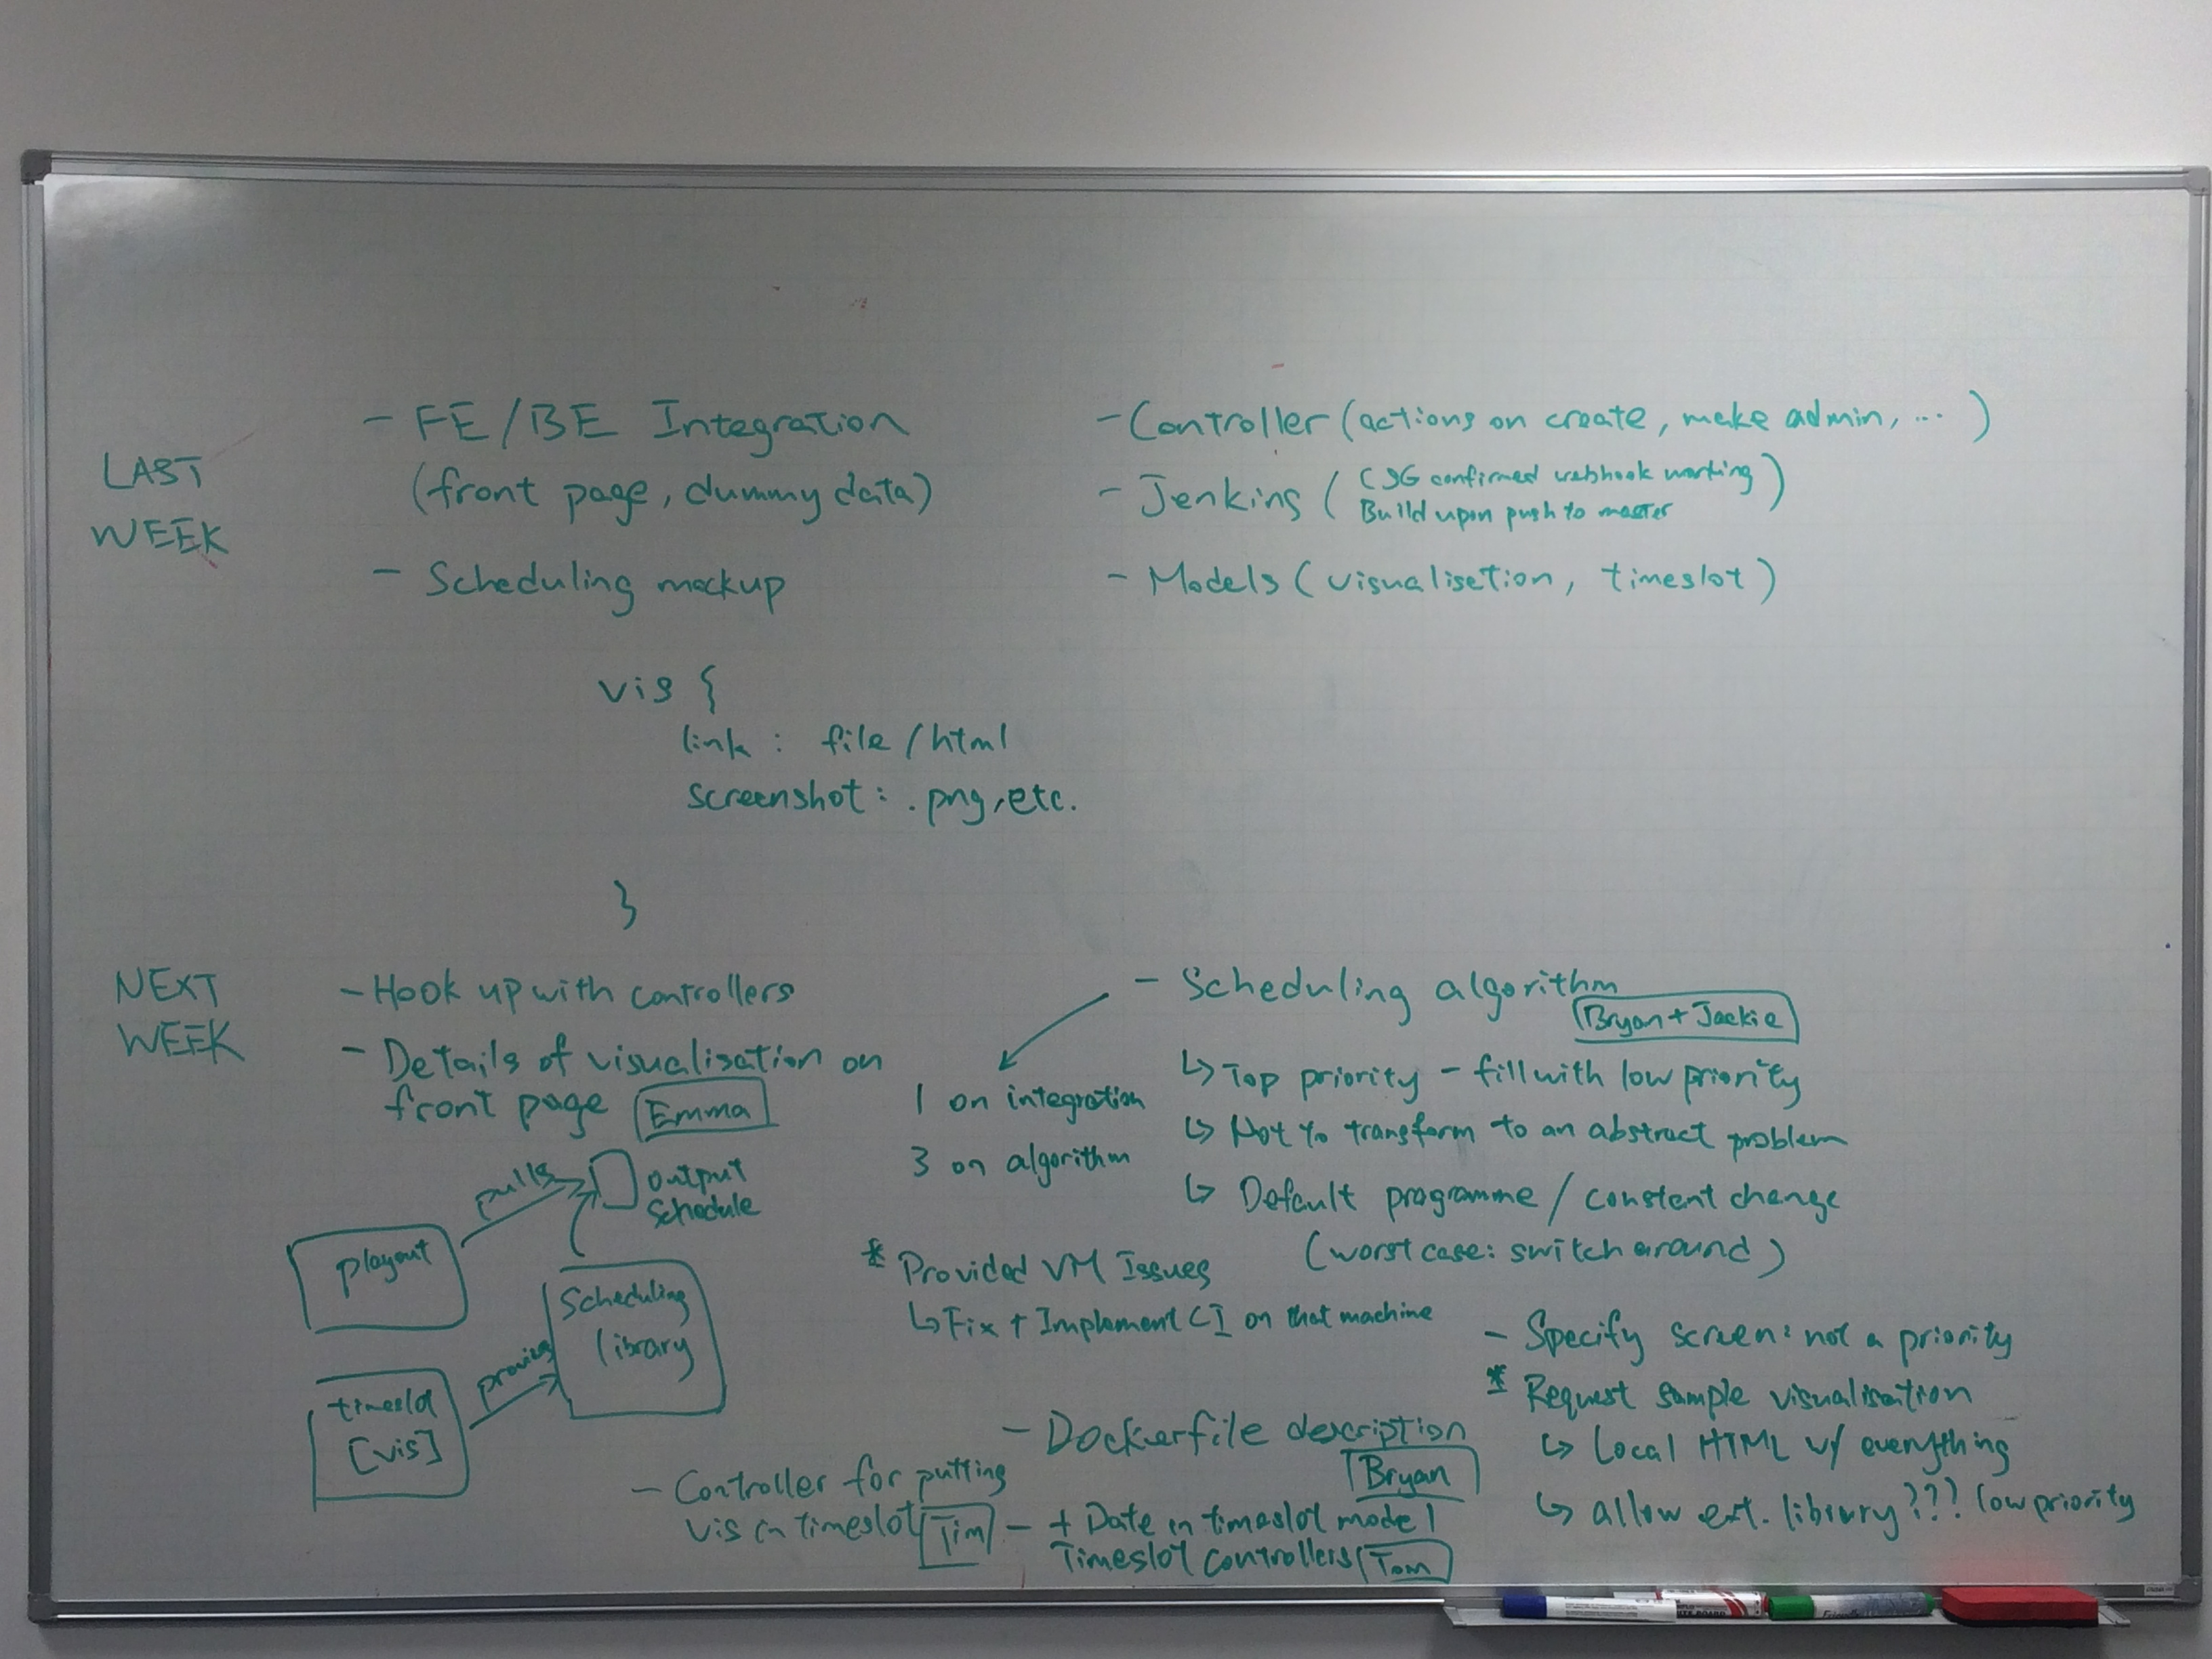
\includegraphics[width = \textwidth, trim = 0 0.4cm 0 1.6cm, clip]{./evaluation/meeting-board2.jpg}
  \end{minipage}
  \begin{minipage}{0.49\textwidth}
    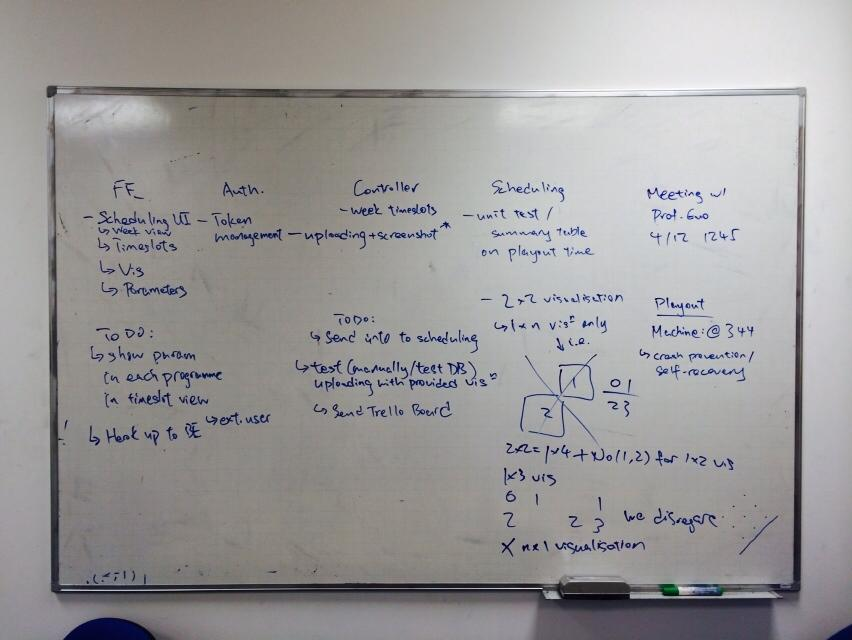
\includegraphics[width = \textwidth, trim = 1.2cm 1.5cm 1.2cm 2.5cm, clip]{./evaluation/meeting-board.jpg}
  \end{minipage}
  \caption{Meeting notes with group progress and feedback from David (our supervisor)\\
                    after sprint cycles 2 (left) and 4 (right).}
  \label{fig:meetingboard}
\end{figure}

Furthermore, with the aid of Jenkins we are able to give our supervisor
the address of our ``release VM'', where he can see the latest working 
version of the project. From this, David can constantly evaluate
and provide feedback on our project features through all stages of development.

\subsection{Feedback handling}
Upon receiving feedback from our stakeholders, mainly from our supervisor,
we handled them depending on their nature:

\begin{itemize}
  \item Change in minor details of a feature/ design: \\
        Usually happening in prototype stage, they include changing font
        size/colour and displaying some extra information on a screen.
        With knowledge that it takes minimal time (within a few hours) 
        to implement, we took the absolute majority of such suggestions
        and fit these XS-items in the next iteration.
  \item Introduction of new, peripheral features: \\
        These includes features that are related but not essential for our
        three main components (submission, moderation/scheduling and playout):
        multiple default playout lists, play videos with 
        linked themes consecutively, buttons to copy and paste previous
        timeslots, etc. \\
        Due to limited time, we chose to integrate only
        one or two small-sized features with our planned implementation.
        The rest of the suggested features was put on a ``extra feature" list,
        which we only consider after a basic version of the main components
        are completed. This ensures that we can produce a minimal
        product before our planned deadline.
  \item Major changes in feature implementation: \\
        As a result of differing assumptions, the feedback necessitates us to
        change what we have implemented. An example would be the team being 
        required to reprioritise the rules in the scheduling algorithm. 
        In these case, we have spent a significant portion of the weekly
        meeting to clarify the assumptions our supervisor is making and try 
        to bring them together with what we have assumed and done.
        These feedback have resulted in some or all of the codes
        being scraped yet a product which is more useful to stakeholders.

\end{itemize}

In any cases, we have clearly communicated with the one who provided the
feedback with justification on our decisions. For example, we have told
our supervisor that we are happy
to take the request to add a button which copies
previous timeslots as we rate it as a S-sized task which can fit in the
planned iteration, but the request for linked videos to be scheduled to 
playout consecutively would delay our plans and thus should only be considered
after the entire system is implemented minimally.


\section{Product Requirement, Value \& Impact}
In the first week of beginning our project, we met with our supervisor 
David to draw out the initial components. Initially, these were general
requirements including:

\begin{itemize}
  \item Stakeholder requirments resembling user stories (e.g.
        a user is allowed to submit scientific visualisation and/or 
        advertisements, as well as to state preference(s) on playout).
  \item System/Interface requirements - what user should expect it could do
        based on the user stories above (e.g. The scheduling system should
        schedule items to play out in rotation, so passersby would not be
        bored by ``fixed" playout).

\end{itemize}

\begin{figure}[H]
  \centering
    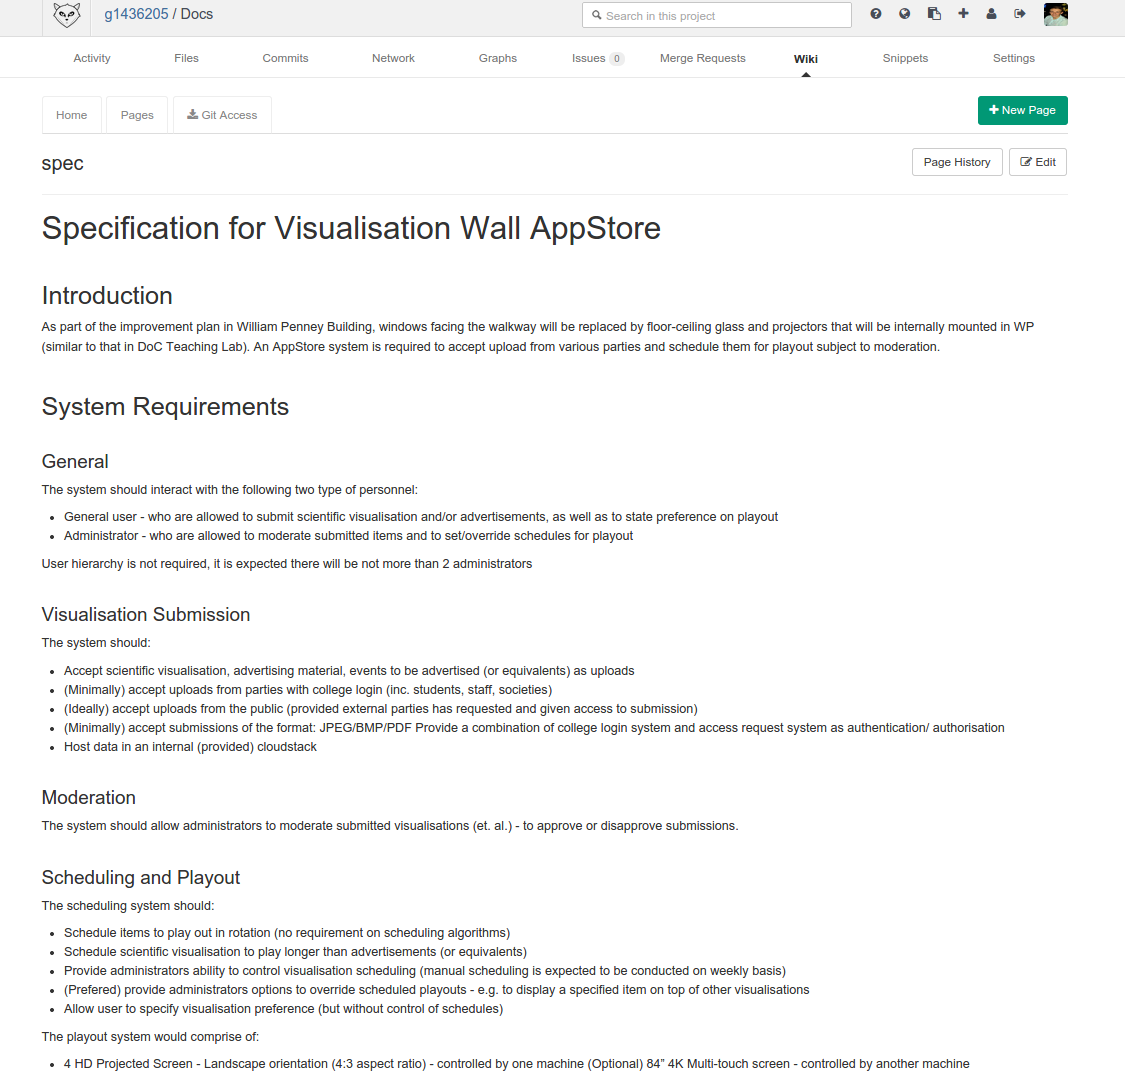
\includegraphics[width = 0.9\textwidth, trim = 0 15cm 0 5cm, clip]{./evaluation/specs.png}

  \caption{Initial specifications (partial) on shared repository.}
  \label{fig:specs}
\end{figure}

In the following weeks, we then clarified and expanded these requirements as 
a group. This allowed us to discuss implementation and technical details
of specific features.

\subsection{Value Proposition}
We also further clarify our understanding on stakeholders and how our system
creates value for them via multiple value proposition canvasses. Figure
\ref{fig:valpropcanvas} shows the canvas for Imperial Data Science Institute,
which our supervisor is associated with. It includes a customer profile
containing list of jobs, gains and pains, and corresponding products/services,
gain creators and pain relievers (value map). Some of the gains/pains
of the institute, along with their creators/relievers are as follows:

\begin{itemize}
  \item Gain: makes the walkway more interesting
        (by showing visualisations to passersby)
  \item Pain: requires a large amount of visualisations
        (relieved by inviting users to submit visualisations)
  \item Gain: creates income opportunities
        (by showing adverts)
  \item Pain: attracts inappropriate submissions from users
        (relieved through admin moderation)
\end{itemize}

The canvasses enables us to disregard features that deliver low or no value
and make more reasonable assumptions about our stakeholders. We believe the
later has resulted the team less pain when we begin our validation, detailed
in section \ref{sec:validation}.

\begin{figure}[H]
   \begin{center}
      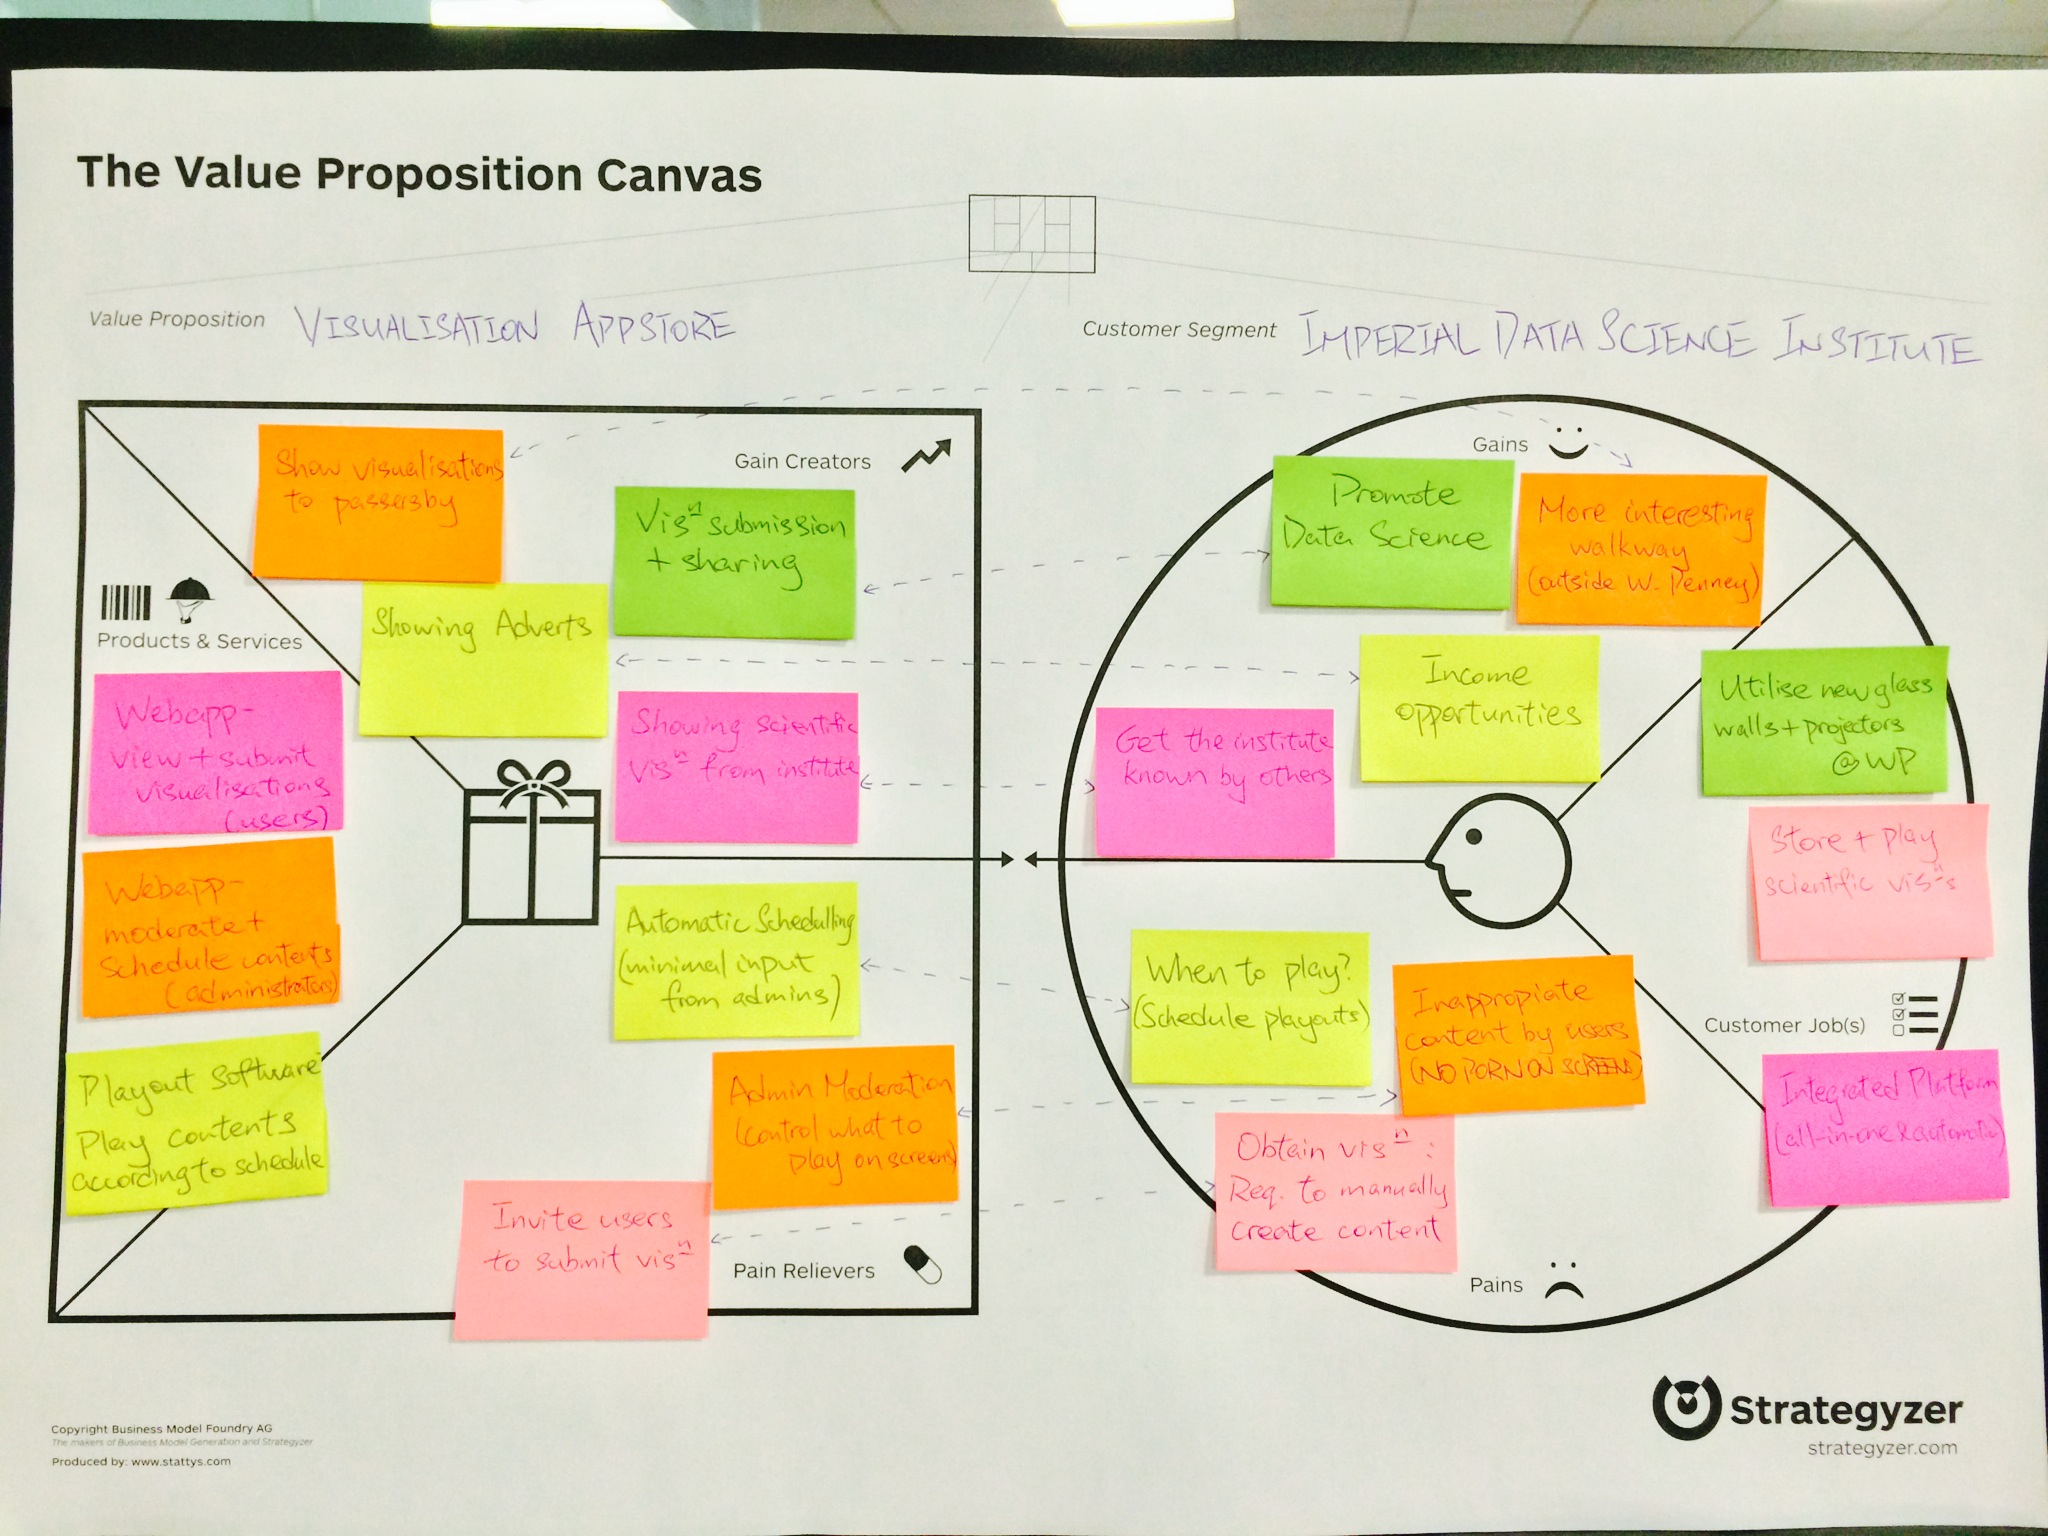
\includegraphics[width = 0.9\textwidth, trim = 1cm 6.5cm 1cm 4.5cm, clip]{./evaluation/value_prop_canvas.jpg}
   \end{center}
   \caption{Value proposition canvas for our client (Imperial Data
            Science Institute).}
   \label{fig:valpropcanvas}
\end{figure}



\section{Task Management}
%TODO: if required to expand



During development, we are constantly looking at the requirements for 
all of our stakeholders, which 
we have stored in a shared document. In our weekly scrums, we have 
presented the work we have done and discuss whether the project is on the 
right track.



We have been prioritising tasks using our Trello board with different
columns. In addition to this, we have been constantly communication both 
in person and online, to make sure members are implementing assigned tasks
in appropriate times. We have been actively encouraging use of the Trello 
board to update the group when tasks have been completed. This way, 
we don't have to constantly ask or look at code to see if a feature has 
been implemented. If appropriate, group members working on the backend
have been using an internal wiki on gitlab to provide information about
routing, controller actions and parameters. 


\begin{figure}[H]
  \begin{minipage}{0.49\textwidth}
    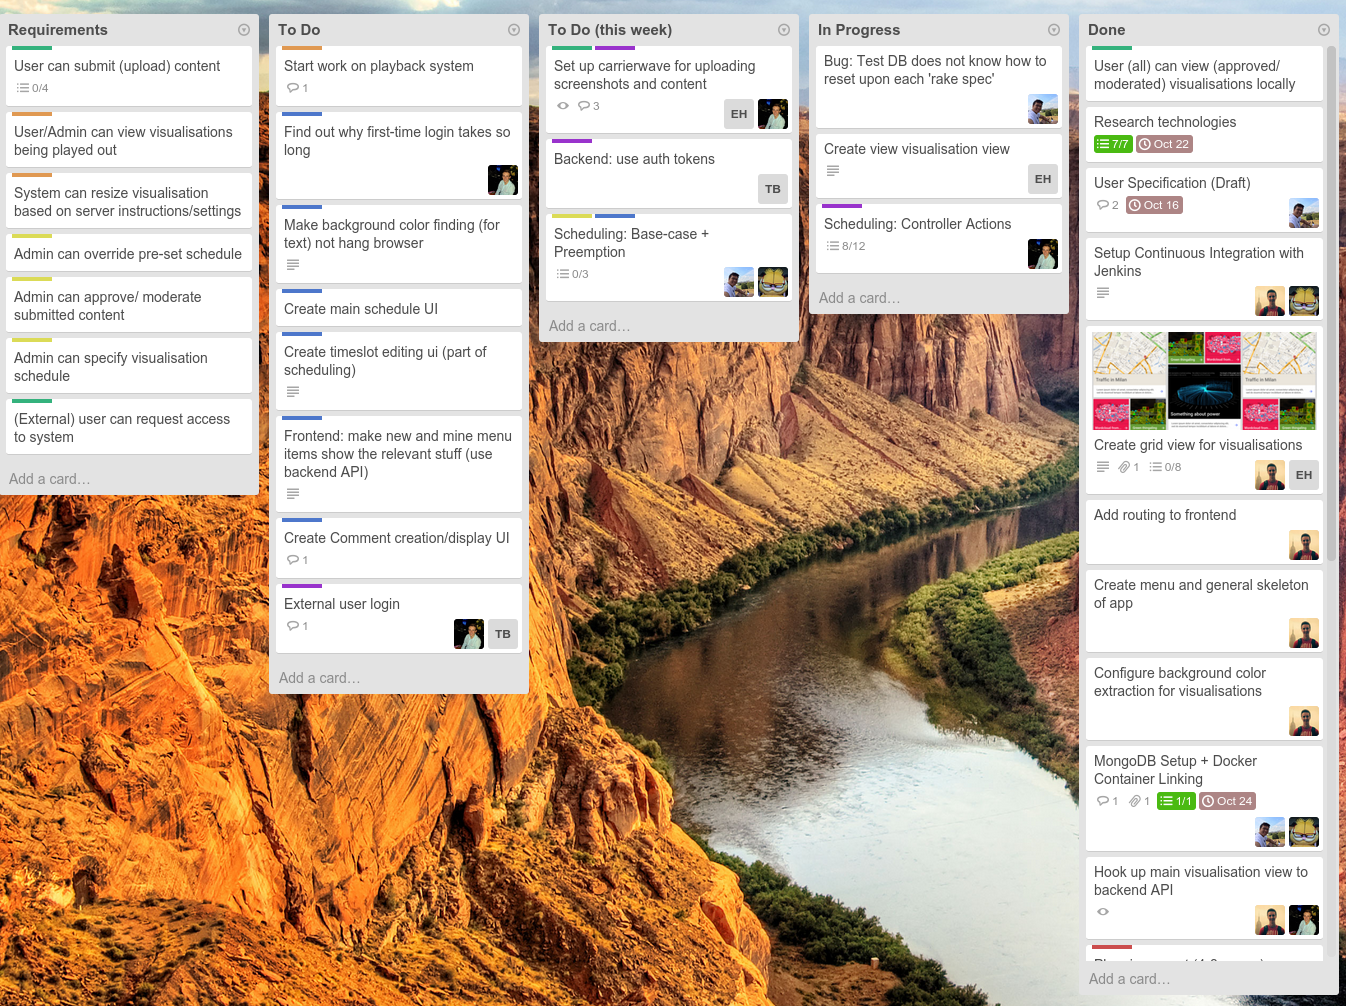
\includegraphics[width = \textwidth]{./evaluation/trello-columns.png}
  \end{minipage}
  \begin{minipage}{0.49\textwidth}
    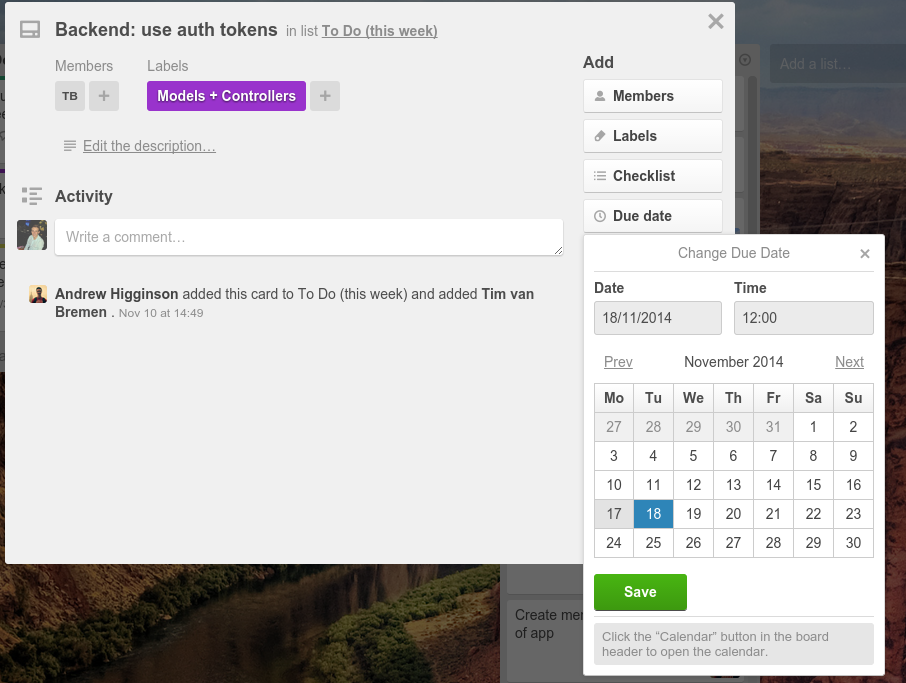
\includegraphics[width = \textwidth]{./evaluation/trello-due-date.png}
  \end{minipage}
  \caption{Priority columns on our Trello board (left) and\\
           Setting a due date for a particular task (right).}
  \label{fig:trello}
\end{figure}


\subsection{Story Splitting}
While some of the requirements require only a few hours effort. We believe
it would be highly unlikely to be able to implement some of the features within an
iteration. In such cases we have splitted the features into multiple units and
implement them in different iterations based on their priority.

An example would be on the user story
 "As a user, I want to access the platform via a set of
credentials so that I can upload visualisation (user)/ perform moderation and
scheduling (administrator)". We consider this to be technically challenging to
be completed in one week if we consider all possible users, yet other features,
such as scheduling and moderation, would require a working version of access
control. As a result, we decided to split it into:

\begin{itemize}
  \item As an internal user (student/staff at Imperial), I want to access the 
        platform via college login so that I can upload/ moderate and schedule
        without memorising an extra set of credentials.
  \item As an external user, I want to access the platform via some kind
        of access request system so that I could participate in visualisation
        sharing as well. 
\end{itemize}

While being reduced in size, splitting the story has also helped us to 
further understand the needs of different groups of users. 
We have decided to implement the former requirement
first as some of our team members have had experience on working with college
login system, allowing the requirement to be fulfilled in shorter time.
The later requirement were then scheduled
to be carried out in parallel with the mentioned features.

\subsection{Spikes - Experiments with new technologies}
Throughout development, we have also devote a small proportion of time to
experiment on technologies involved in later iterations. This allows us to
better understand the complexity we will face and react accordingly.

While we have scheduled to implement the playout system in iterations 5 and 6
(the last two iterations),
investigation on relevant technologies, including QT and its adapters, were
made from iteration 2. By performing preliminary research, it allows 
us to confirm that 2 weeks would be a reasonable estimate in system 
implementation. Furthermore, we believe the investigation would result 
in a more gentle learning curve, and reduces the risk for development 
grinding to a halt as team members would
at least have some basic knowledge on QT and some code segments are produced.

Not all spikes brings good news - investigation on Kerberos login libraries has
revealed that the adapter for Flask (with Python) is actually broken.
Though being required to scrap the entire implementation, the spike allows us
to switch development language early and thus avoids incurring high 
cost further into development.


\section{Building the right thing - Assumption Validation} \label{sec:validation}
Given the tight time constraints for the entire project, we agreed to collect
user feedback as soon as the project commences. This ensures the team
is building the right thing which our client needs.

\subsection{UI mockups/ prototypes} \label{sec:uimockup}
A release cycle in our project generally takes the following form. Before
implementing a particular part of our project, we begin with creating
mockups (figure \ref{fig:mockup}). These are relatively quick to produce
and allow us to quickly think through the design of our project,
with being tied down to any implementation details which would affect
our thinking. After completion, we then show the mockups to the main
stakeholder in the project, our supervisor David, who gives us
feedback/changes. For example, he mentioned that it would be a good if we could 
show the priorities associated with each visualisation in timeslot view, 
even if the visualisation is not selected after viewing the mockups.


Once a general design is settled on, within that week's
sprint cycle, we complete the main implementation of the UI, but only do 
so up to the point of it being useful to show how it would be used. It is
not yet interfacing with the backend, and hence small changes at this 
point are simple to do, with the following week's sprint cycle involving
'hooking' up this UI prototype and our backend.

We also make sure that this prototype is in some way, seeded with some
dummy/representative data, so that it is clear how each part of the project
will operate in practice.

\begin{figure}[H]
   \begin{center}
      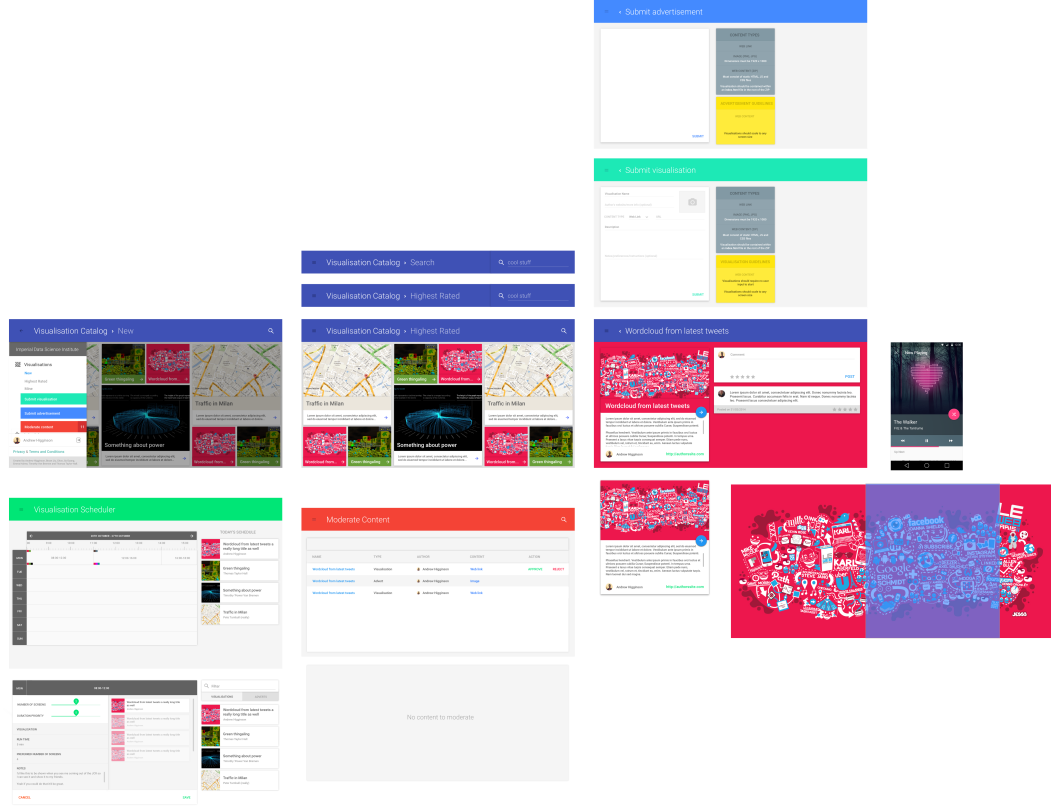
\includegraphics[width = 0.9\textwidth, trim = 0 0 0 0cm, clip]{./evaluation/mockup.png}
   \end{center}
   \caption{Mockups on User Interface}
   \label{fig:mockup}
\end{figure}

\subsection{Requirements on intangible ideas}
Compared to User Interfaces which user can see and feel, we believe 
uncovering the client's assumption on playout scheduling via mockups or 
prototypes would not be feasible as the algorithm is mainly rule-based.
We instead deliver our ideas with illustrations on whiteboard and
capture feedback from our supervisor.

Throughout discussions we have uncovered several assumptions, with one of them
expecting the scheduling algorithm to ensure playout time is 
directly proportional to metric set by administrators. In response,
we have created additional unit tests to incorporate such requirements 
in our scheduling algorithm.

\begin{figure}[H]
  \begin{minipage}{0.46\textwidth}
      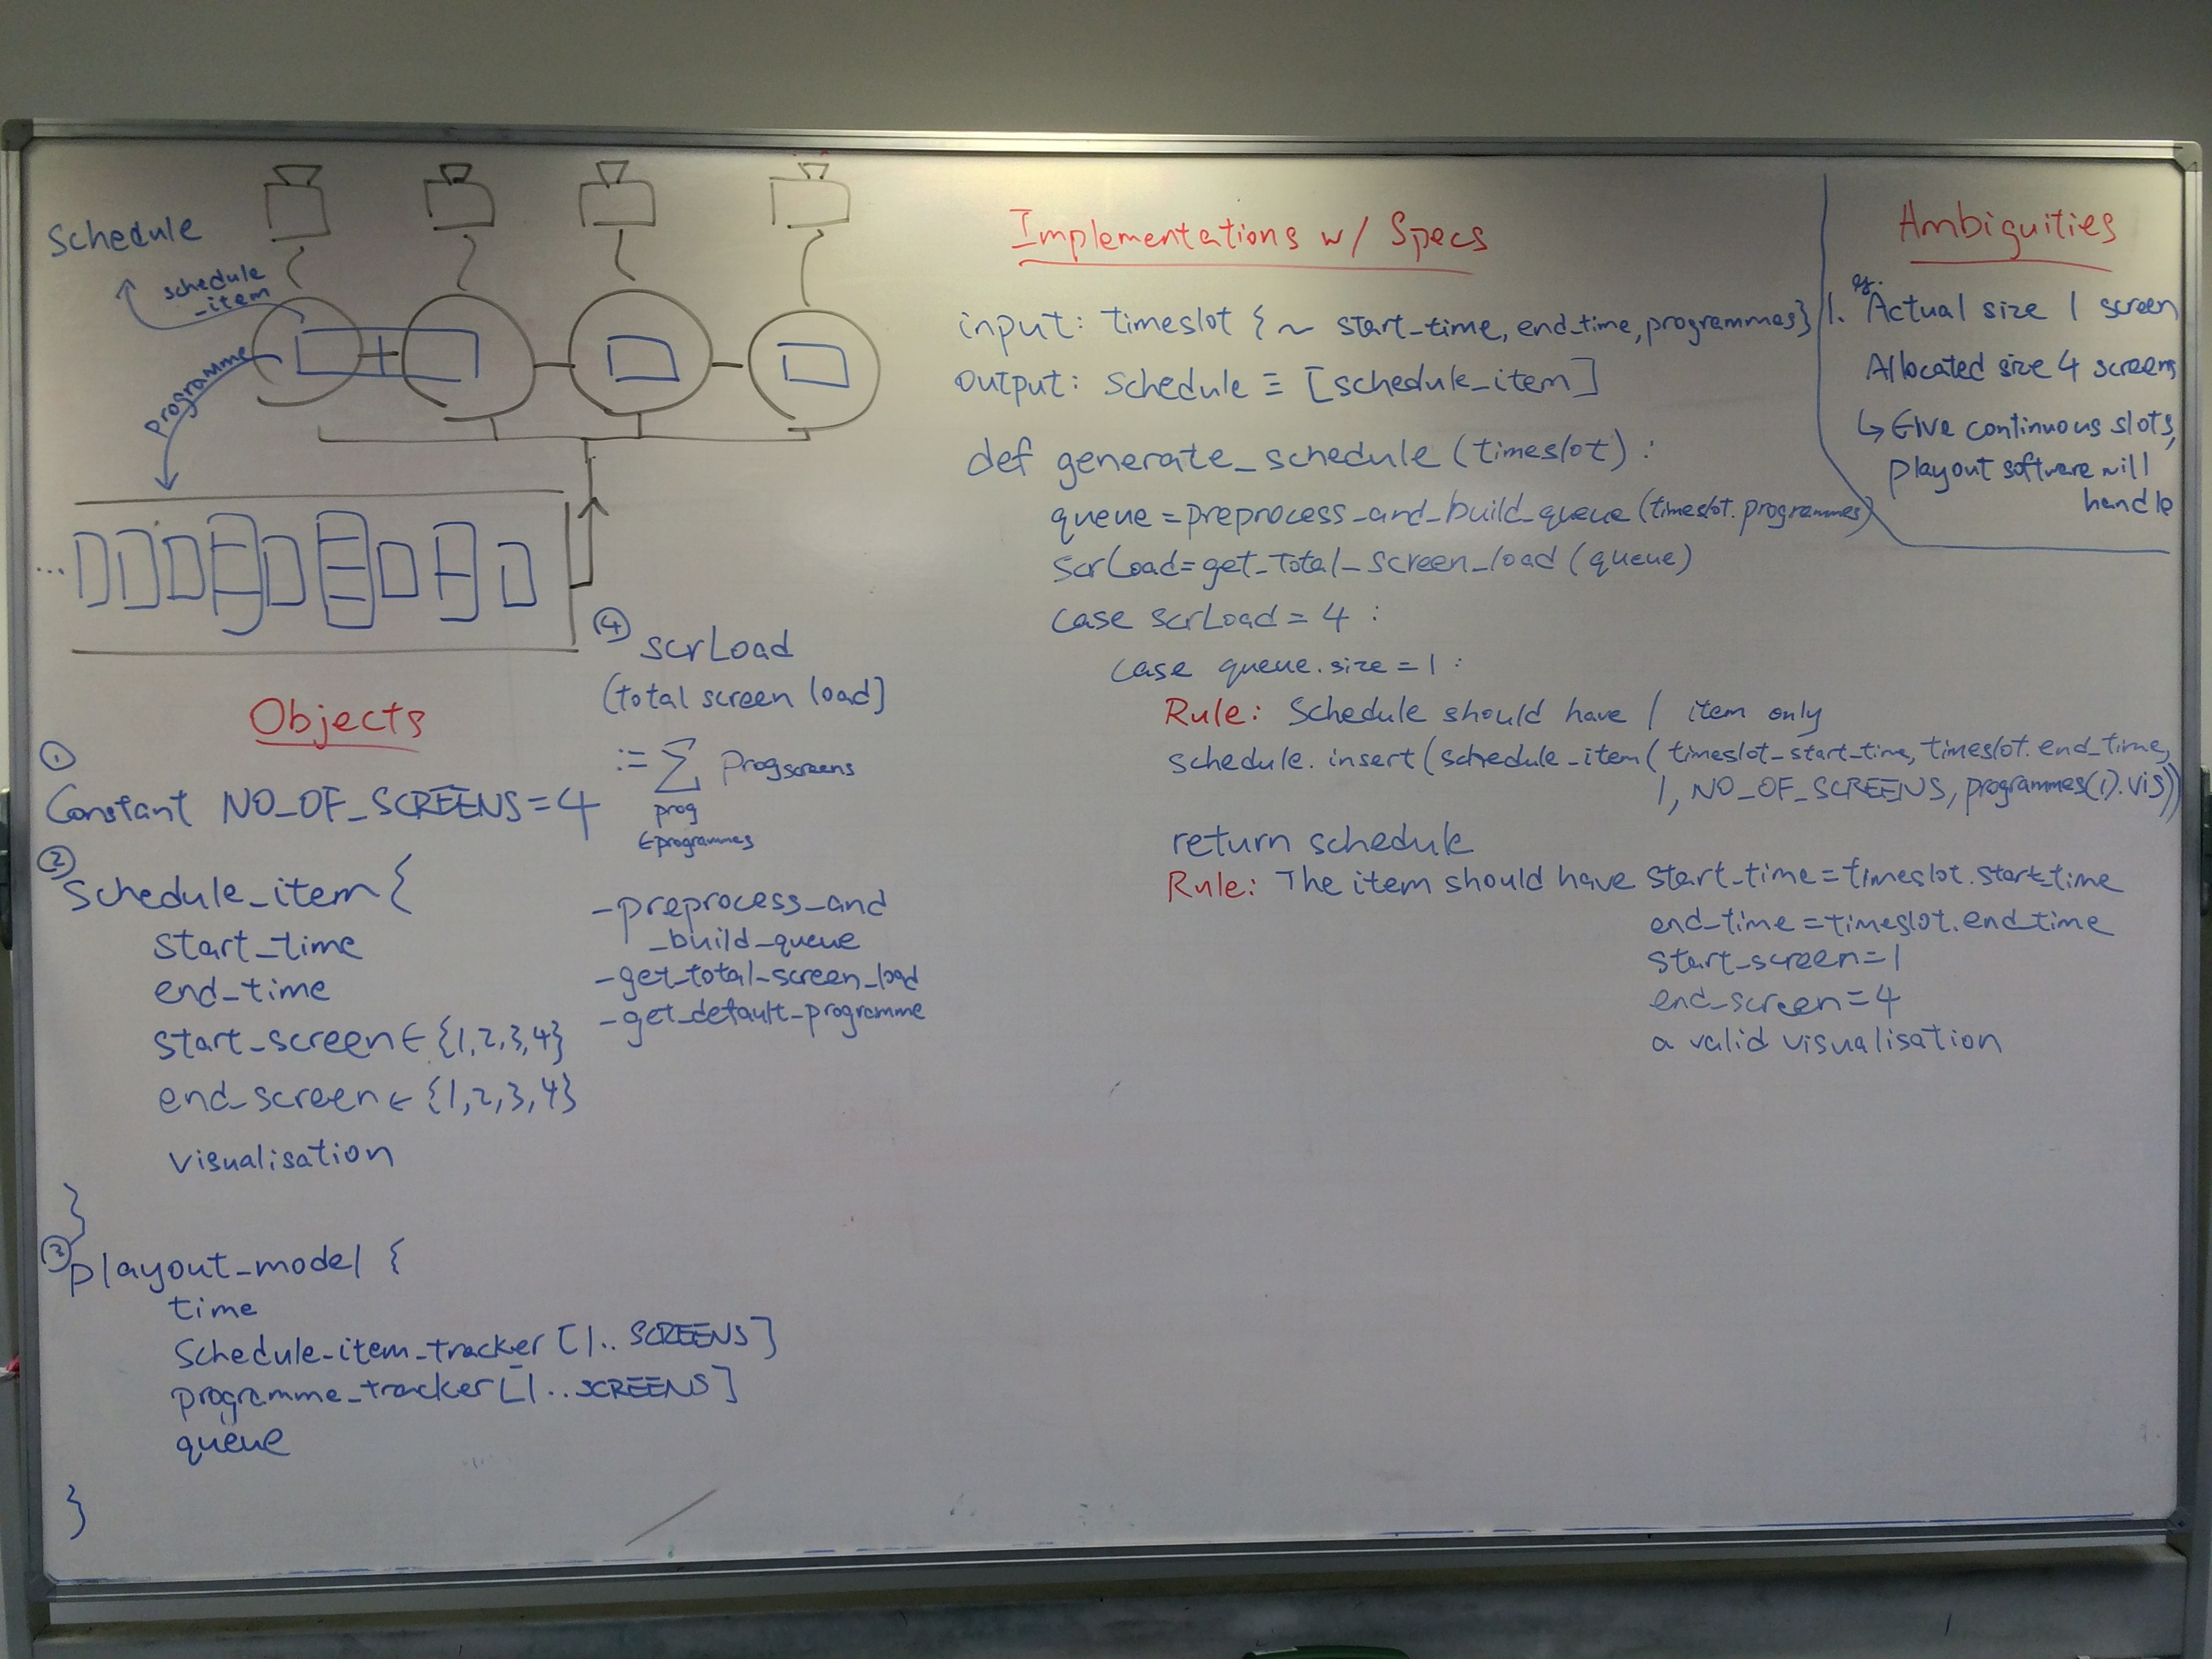
\includegraphics[width = 0.99\textwidth, trim = 0 1cm 0 1.5cm, clip]{./evaluation/scheduling_whiteboard.jpg}
  \end{minipage}
  \begin{minipage}{0.53\textwidth}
      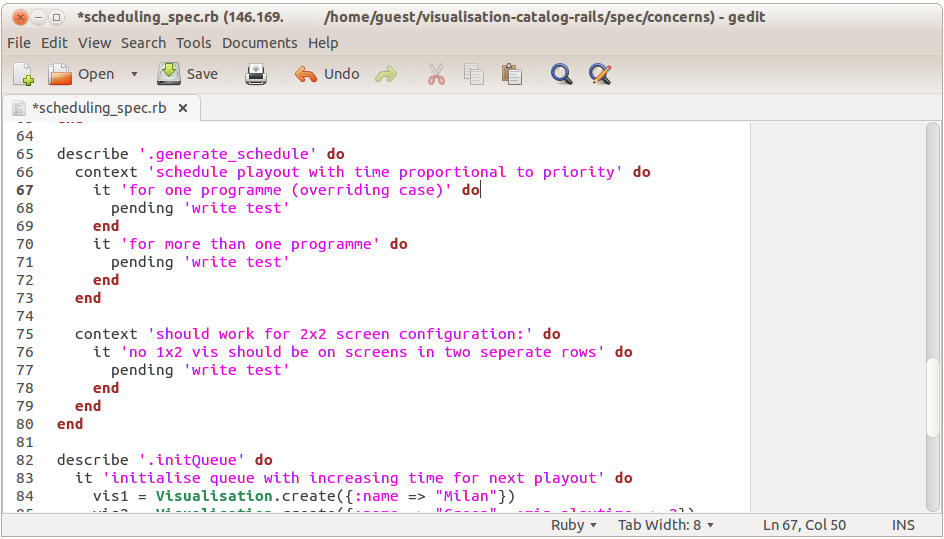
\includegraphics[width = 0.99\textwidth]{./evaluation/scheduling_spec.png}
  \end{minipage}
  \caption{Capturing scheduling requirements on whiteboard (left)\\ and subsequently via RSpec unit tests (right)}
 
\end{figure}

\subsection{User testing}
We have also conducted implicit user tests during demonstrations of new features,
where we ask our supervisor to conduct a task with minimal instruction and guidance
(e.g. to navigate to the visualisation scheduling page and schedule some visualistions
for playout).

Such testing allows us to learn what are obvious to us but obscure to users.
For example, in one of our demonstrations we observed that our supervior 
made multiple pauses when
being asked to navigate to the moderation and scheduling pages. This 
indicates the icon to show the user menu might not be evident to users and
description for menu items might not be clear enough. Based on such observations
we have changed the size of the ``show menu" button, as well as explored the effect
of different link colours on user menu.

We are planning to extend the user to test to cover more users, including staff
and students who would potentially use the platform to submit and 
view visualisations, the second in our list of stakeholders.

\section{Evaluation}
As a group, we are constantly evaluating the correctness of our project by 
unit and system tests after a feature is implemented via RSpec. 



\subsection{Validated learning \& Pivoting}
Producing mockups and prototypes with representative data, as mentioned
in section \ref{sec:uimockup}, and obtaining feedback based on them allows
us to 'pivot' many times, and with minimal overhead
of reimplementation, as it allows us to identify problems, or learn more about
the issue we are trying to solve, before we write large volumes of code which
may end up to be not useful. The fact that we have this lean approach also
\textbf{encourages us} to pivot more often, as there is no reason not to do so.

\subsection{Project progress}
In each 


Quantitively, we can evaluate our project by ticking off our intial 
requirements. Also, we will use the systems ourselves, both from the user 
and administrator perspective, to evaluate the project from both our stakeholders.
This will include uploading of visualisations and viewing other visualisations as a
user, and moderating and scheduling visualisations as an admin.

Using our Trello board and version control, we can see which features have been 
implemented by which group member. To improve our teamwork for future group 
projects, we will sit down as a group and describe our strengths and weaknesses in 
this project.

% TODO: get externals to evaluate, people from data science institute? 

% TODO: stuff from eval lecture

% TODO: metrics: move trello to here



\end{document}
